\section{Versuchsaufbau/-durchführung}
Das verwendete Kugelfall-Viskosimeter ist in Skizze \ref{fig: aufbau} abgebildet. Das mit destilliertem Wasser gefüllte Fallrohr ist mit zwei Messmarken versehen ($s = 100\si{\milli\meter}$\cite{anleitung207}), die eine Geschwindigkeitsmessung über das Weg-Zeit-Gesetz ermöglichen.
Es befindet sich innerhalb eines mit Wasser gefüllten Zylinders, dessen Temperatur über ein Thermostat reguliert wird. Der Zylinder lässt sich um $180 \si{\degree}$ drehen und ist
um einen kleinen Winkel geneigt, sodass ein unkontrolliertes Stoßen zwischen Kugel und Rohrwand vermieden wird. Der Durchmesser des Rohres ist geringfügig größer als jener der verwendeten Glaskugeln.\\
Zunächst wird das Fallen in destilliertem Wasser einer Kugel $\kappa_{Kl}$ mit Radius $R_{Kl}$ bei Raumtemperatur beobachtet, deren Proportionalitätsfaktor $K_{Kl}$ \eqref{eq: eta} aus der
Praktikumsanleitung \cite{anleitung207} bekannt ist. Die Fallzeit $T_{Kl}$, sprich die Zeit zwischen dem Passieren der oberen und unteren Marke,
wird zehn mal gemessen. Hierbei wird jeweils ein Vorgang mit zwei Stoppuhren gemessen und anschließend der Zylinder um $180\si{\degree}$ gedreht, sodass die
Kugel erneut hinab fällt. Danach wird selbiges mit einer zweiten, größeren Kugel $\kappa_{Gr}$ ($R_{Gr} > R_{Kl}$) durchgeführt. Dies ermöglicht später
mittels der Annahme, dass die Viskosität bei konstanter Temperatur gleich bleibt, die Berechnung der Konstante $K_{Gr}$ der zweiten Kugel. \\
Mit Hilfe des Thermostats wird nun die Temperatur der Flüssigkeit im Fallrohr auf zehn verschiedene Werte geregelt und jeweils die Fallzeit der großen Kugel $T_{Gr}$ zwei mal aufgenommen.
\begin{figure}
  \centering
  \fbox{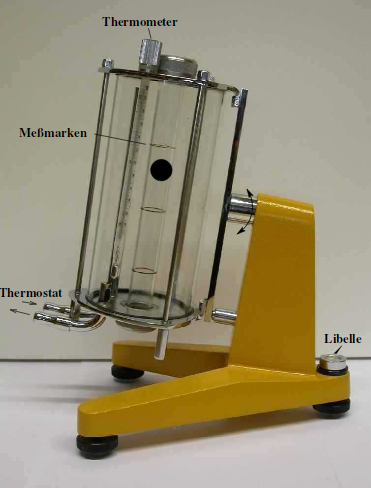
\includegraphics[width = 4cm]{pics/Kugelfallviskosimeter.png}}
  \caption{Kugelfall-Viskosimeter \cite{anleitung207}}
  \label{fig: aufbau}
\end{figure}
